\section{A Proposed Model for Reactive Load Balancing in HPC}
\label{sec:NewModel-ReactLB}
\index{PerfModel!A New Performance Model in HPC}

For modeling the performance of dynamic load balancing, we need to understand the behavior associated with balancing operations. For this, we rely on experiments and profiling information to build the model. To stay consistent with the example in Figure \ref{fig:preli_reactlb_operations} on Page \pageref{fig:preli_reactlb_operations}, we highlight the same illustration for reactive balancing behavior in Figure \ref{fig:perfmodel_reactlb_deterministic_estimation}, but we emphasize in detail the steps when task offloading is performed.\\

Figure \ref{fig:perfmodel_reactlb_deterministic_estimation} can be considered as a profiled information of $8$ processes. The y-axis shows $8$ involved processes ($P = 8$), while the x-axis shows execution progress over time steps (time units) from $0$ until termination. In Figure \ref{fig:perfmodel_reactlb_deterministic_estimation}, before tasks are executed, we assume there is a given distribution of $5$ tasks on each process (formulated by $T_{i} = 5$). The performance of each process is expected to be stable, and total load value is balanced. However, the execution speed of processes $P_{4}$, $P_{5}$, $P_{6}$, $P_{7}$ is slowed down, leading to an imbalance at runtime as Figure \ref{fig:perfmodel_reactlb_deterministic_estimation} reveals. With reactive load balancing, each process is deploying a dedicated thread, \texttt{Tcomm}, which is denoted by the dashed line, and the small triangles on each line illustrate reactive operations. For example, at time $t_{6}$ and time $t_{8}$, tasks from the slower processes are offloaded to the faster processes. In terms of two objective factors affecting the decisions of task offloading, we have:
\begin{itemize}
	\item Imbalance level: points to the effect of slowdown on the imbalance ratio.
	\item Reasonable task migration: points to the effect of balancing approach and overhead in balancing operations \& task migration on the offloading decision.
\end{itemize}

\begin{figure}[t]
  \centering
  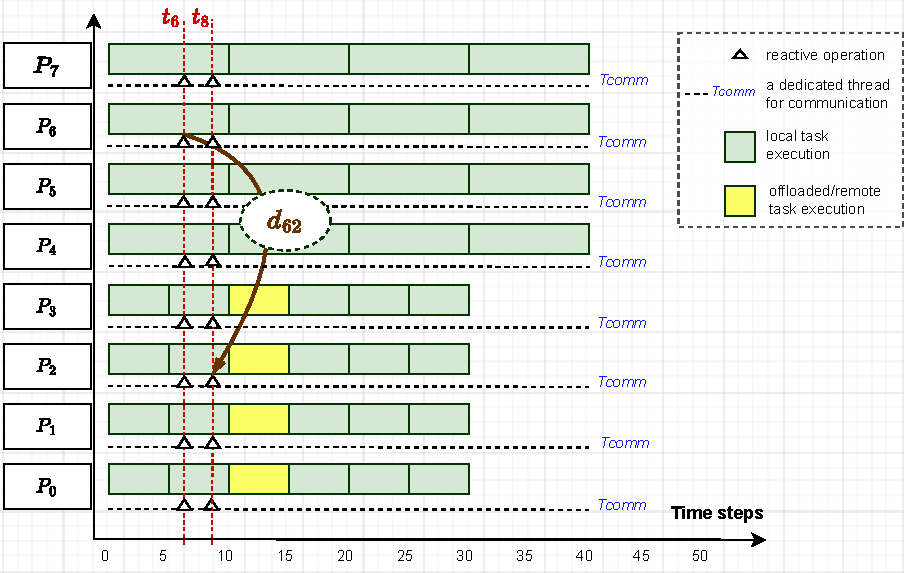
\includegraphics[scale=0.65]{./pictures/perf_analysis_model/perf_illustration_reactlb_behavior_for_perf_model.pdf}
	\caption{An illustration about the analysis of reactive load balancing based on deterministic estimation.}
	\label{fig:perfmodel_reactlb_deterministic_estimation}
\end{figure}

Following the slowdown affecting execution speed, we formulate the speed of corresponding processes such as speed $S_{P_{0}}$, $S_{P_{1}}$, $S_{P_{2}}$, ..., $S_{P_{7}}$. The total load value of each processes is formulated by load $L_{0}$, $L_{1}$, $L_{2}$, ..., $L_{7}$. In the case of balance, all speed values and their total load values are approximately similar. In the case of imbalance, some speed values are affected by a slowdown factor which we denote by $Slow_{i}$. If $Slow_{i} < 1.0$, it can make the execution speed of process $P_{i}$ slower. For example, the expected speed of process $P_{i}$ is $S_{P_{i}} = 1.0$ (can be simplified as $1$ task/time unit). When it is slowed down by $50\%$ ($\times 0.5$), the execution speed would be $0.5$ task/time unit. Otherwise, if $Slow = 1.0$, the execution speed is not changed. For mapping slowdown to the execution time of a task, assuming a time unit is in seconds, then the execution of a task takes one second ($1s$) if the speed $S_{P_{i}}$ is $1.0$ task/second. If $Slow_{i} = 0.5$ affects the speed $S_{P_{i}}$, that task needs $2s$ to be finished.\\

In a specific context, when we can analyze the impact of slowdown factor on imbalance levels by keeping a given distribution of tasks and a number of involved processes, then varying slowdown factor as well as the number of slowdown processes. For changing the $Slow_{i}$ values, we can formulate its impact on speed $S_{P_{i}}$ and load $L_{i}$ by Equation \ref{eq:slowdown_impact_speed_and_L}.

\begin{equation} \label{eq:slowdown_impact_speed_and_L}
\begin{split}
	Slow_{i} & \overset{impact}{\rightarrow} S_{P_{i}}: S_{P_{i}} \times Slow_{i} \\
	Slow_{i}' = \frac{1}{Slow_{i}} & \overset{impact}{\rightarrow} L_{i}: L_{i} \times Slow_{i}'
\end{split}
\end{equation}

In Equation \ref{eq:slowdown_impact_speed_and_L}, $Slow_{i}$ affects directly execution speed, and the value of $S_{P_{i}}$ can be decreased. $Slow_{i}'$ affects directly the total load value at the end; therefore, the value of $L_{i}$ can be increased. Taking the case in Figure \ref{fig:perfmodel_reactlb_deterministic_estimation} for instance, we assume the total load values of all processes are multiplied with an array of $Slow_{i}'$ values. Then, the slowdown at runtime makes them unbalanced and $R_{imb}$ is calculated along with $Slow_{i}'$. Note that load $L_{i}$ without performance slowdown are expected equally; therefore, we can assume that load $L_{0}$ $\approx$ $L_{1}$ $\approx ... $ $L_{7}$ and $\approx$ $L$. In average, the total load values and imbalance ratio can be calculated by Equation \ref{eq:unexpected_imb_8_ranks}.

\begin{equation} \label{eq:unexpected_imb_8_ranks}
\begin{split}
	L_{max} &= \text{max}(L_{0} \times Slow_{0}', ..., L_{7} \times Slow_{7}') \\
	L_{avg} &= L \times \frac{Slow_{0}' + ... + Slow_{7}'}{P}, \text{where } L \approx L_{0} \approx ... \approx L_{7}) \\
	R_{imb} &= \frac{L \times Slow_{max}'}{L \times \frac{Slow_{0}' + ... + Slow_{7}'}{P}} - 1\\
	        &= \frac{P \times Slow_{max}'}{\sum_{i=0}^{P-1} Slow_{i}'} - 1
\end{split}
\end{equation}

The following estimation analyzes two common cases of slowdown effects.\\

\begin{figure}[t]
  \centering
  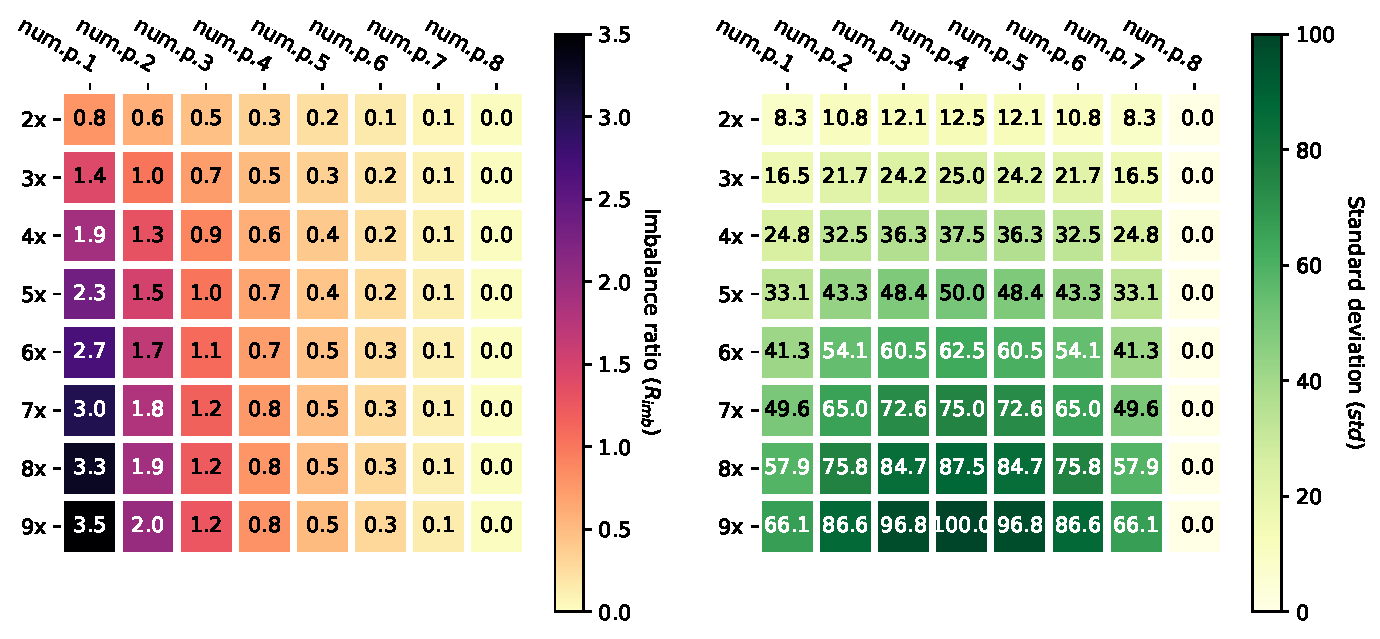
\includegraphics[scale=0.625]{./pictures/perf_analysis_model/perf_heatmap_slowdown_impact.pdf}
	\caption{The impact of slowdown values on load imbalance ratios.}
	\label{fig:heatmap_slowdown_impact}
\end{figure}

\noindent \textbf{Case 1:} Slowdown remains constant during execution, and this happens on some processes, which are called slowdown processes. The slowdown values among processes can be different. However, to easily show the slowdown effect changing over its values and over the number of involved processes, Figure \ref{fig:heatmap_slowdown_impact} highlights an estimation by two heatmaps, where one on the left shows the heatmap color of imbalance ratio ($R_{imb}$) and one on the right shows the color of standard deviation ($std$). Each figure is labeled on the horizontal axis with the number of slowdown processes (such as $num.p.1$, $num.p.2$, ..., $num.p.8$), and on the vertical axis with the factor of slowdown (such as $2\times$, $3\times$, ..., $9\times$). The experiments in Figure \ref{fig:heatmap_slowdown_impact} are stayed with $8$ processes. As an example, $num.p.1$ indicates that one of $8$ processes is slowed down, while $2\times$ indicates the slowdown factor in that process is $2$ times compared to the stable processes. Depending on the color of the heatmap, we determine an imbalance ratio corresponding to a standard deviation. For example, in the case of $num.p.1$ and $2\times$, the imbalance ratio is $0.8$, corresponding to a standard deviation of $8.3$. The value of standard deviation indicates load dispersion between different processes.\\

\begin{figure}[t]
  \centering
  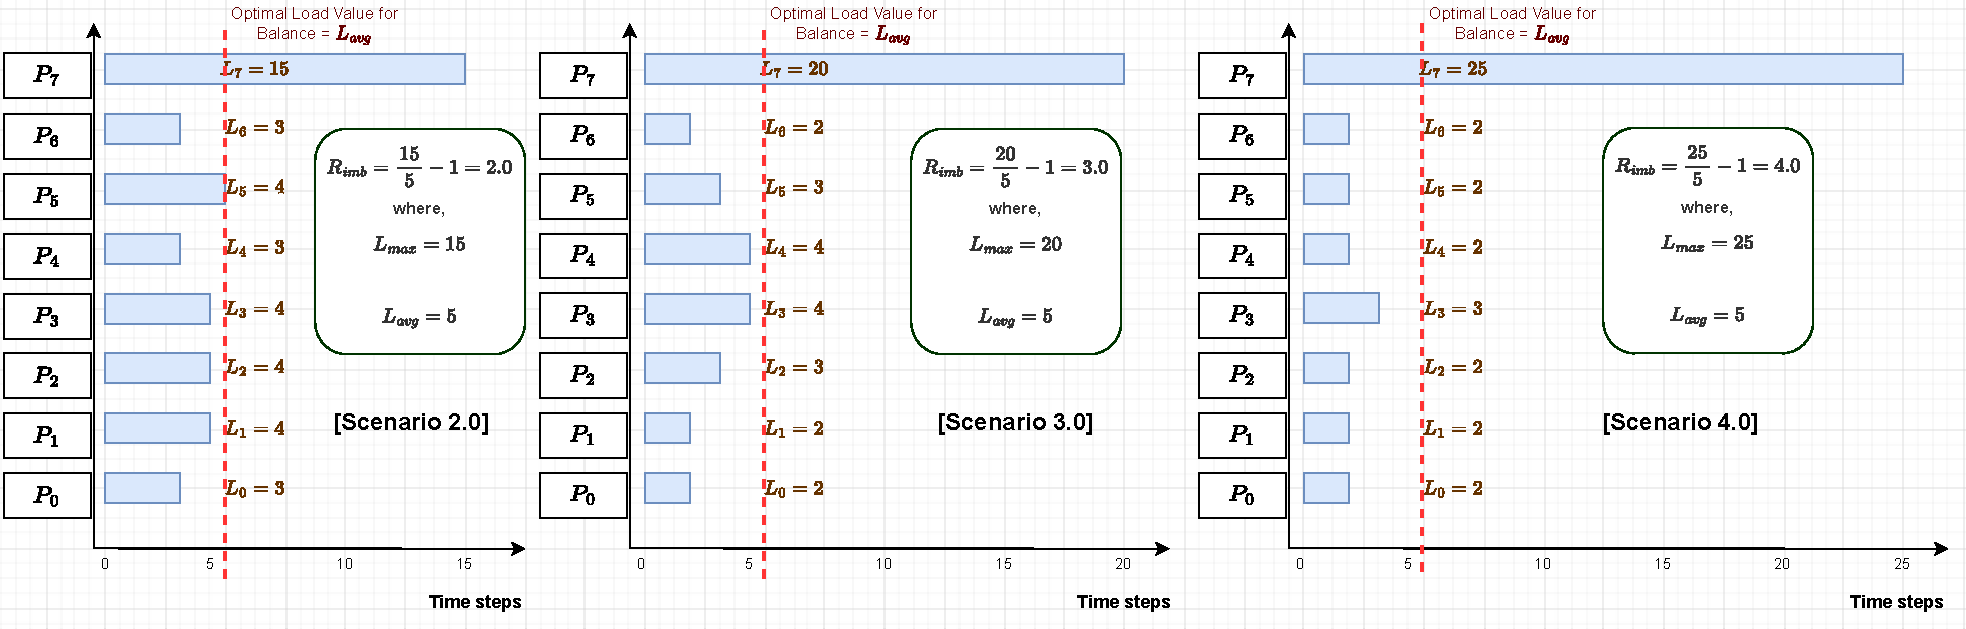
\includegraphics[scale=0.45]{./pictures/perf_analysis_model/perf_analysis_deterministic_model_imb_cases.pdf}
	\caption{Three imbalance scenarios when only one process is slowed down.}
	\label{fig:three_imb_situations_with_one_slow}
\end{figure}

As can be seen, bad situations occur when slowdown cases happen only in a few processors/cores corresponding to the mapped processes or threads. The worst in this example is when one process is significantly slowed down. Figure \ref{fig:three_imb_situations_with_one_slow} highlights three imbalance scenarios with $R_{imb}$ $=$ $2.0$, $3.0$, $4.0$ (named accordingly Scenario 2.0, Scenario 3.0, Scenario 4.0), where only process $P_{7}$ is slowed down. If tasks are migrated to balance the load, only process $P_{7}$ should offload tasks to others.\\

\noindent \textbf{Case 2:} Slowdown is unpredictable, where $Slow_{i}$ is varied during execution. Assume that the execution example is still stayed with $8$ processes as in Figure \ref{fig:perfmodel_reactlb_deterministic_estimation}, we perform the execution running over $100$ iterations, where the slowdown values are randomized over each iteration. Figure \ref{fig:randomized_slowdown} shows an estimation of Case 2 with both lines: imbalance ratio ($R_{imb}$) and standard deviation ($std$). The x-coordinate denotes the indices of iterations; the left and right y-coordinates denote imbalance ratio and standard deviation respectively. If the uncertainty of slowdown is high, this leads to a challenge in load prediction and dynamic load balancing. Particularly, it is difficult to propose a good strategy for migrating tasks.\\

\begin{figure}[t]
  \centering
  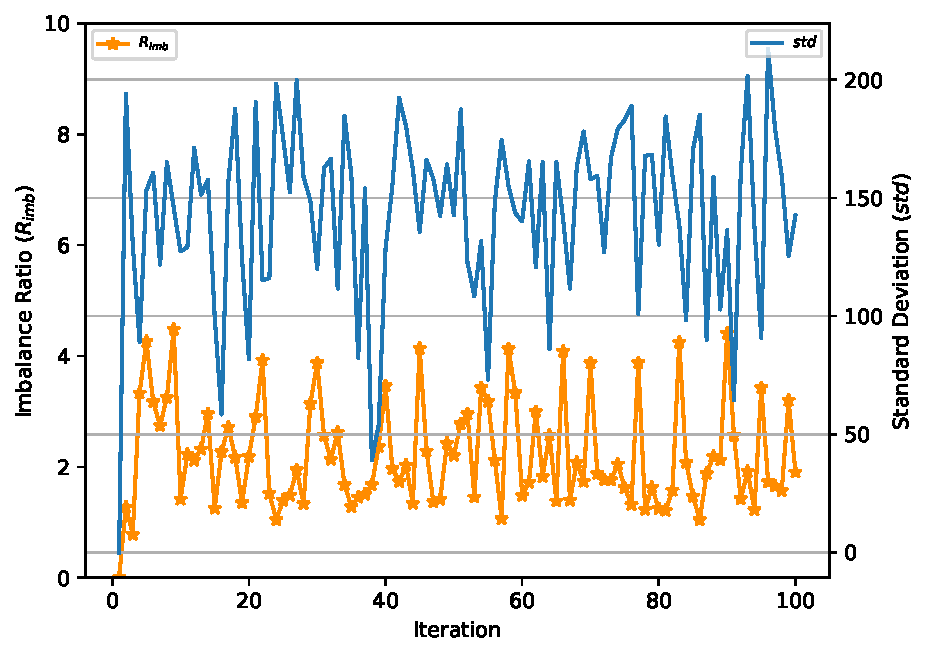
\includegraphics[scale=0.45]{./pictures/perf_analysis_model/perf_double_line_random_slowdown.pdf}
	\caption{Randomized slowdown and unpredictable imbalance ratios over 100-iterations execution.}
	\label{fig:randomized_slowdown}
\end{figure}

In practice, Case 1 and Case 2 might be overlapped except when the fluctuation level of Case 2 is too high. Case 2 usually happens when our computing resources are over-subscribed by sharing between different programs simultaneously. Otherwise, Case 1 occurs more often in parallel compute clusters because of the inherent variation of chip design today, such as variation in power and temperature of the chips. Acun et al. \cite{acun2016variturboboost} have shown similar experiments like Case 1 caused by the variation among processors on the Turbo Boost-enabled supercomputers (an execution time difference of up to $16\%$). The other works from \cite{weisbach2018hwvariation} \cite{tuncer2019onlinediagvar} have introduced the methods and tools to characterize hardware performance variation, even reproduce performance variations for research purposes \cite{ates2019hpas}. In addition, not only CPUs, similar analyzes are also performed on current GPU architectures \cite{yoshida2022perfvargpu}.\\

%The estimation of these two cases shows how much slowdown can impact the level of load imbalance.\\ 

Following a given imbalance level, the next subsection introduces how the overhead in balancing operation and task migration can affect the decision of task offloading. Typically, we show an estimation of the maximum number of tasks that need to be exchanged to balance the load in a specific situation.

% ----------------------------------------------------
% Deterministic Estimation in average
% ----------------------------------------------------
\subsection{Deterministic Estimation} \label{subsec:deterministic_estimation}

Deterministic estimation aims at calculating on average for how many tasks can be offloaded. For example, we have a given imbalance ratio, a number of involved processes which we know overloaded and underloaded processes. Then, according to the overhead of task migration, we can estimate how many tasks should be migrated. The model for deterministic estimation provides an overview in advance about how task migration is limited in a specific case and in a specific system.\\

% ---------------------------------
% insert an inline figure here
% ---------------------------------
\begin{figure}[t]
  \centering
	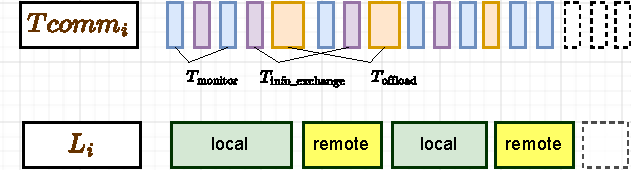
\includegraphics[scale=0.8]{./pictures/perf_analysis_model/perf_inline_fig_Li_and_Tcomm.pdf}
	\caption{Three main operations driven by reactive load balancing and total load value afterward.}
	\label{fig:detailed_Tcomm_operations_and_L}
\end{figure}

Before a task is migrated, there are three main operations driven by the reactive load balancing approach, including monitoring execution status, exchanging status, and offloading tasks. These operations are performed by $Tcomm$ at runtime and shown as $T_{\text{monitor}}$, $T_{\text{info\_exchange}}$, and $T_{\text{offload}}$ in Figure \ref{fig:detailed_Tcomm_operations_and_L}. The line of $Tcomm_{i}$ illustrates balancing operations according to process $P_{i}$. Because these three operations cause the most overhead that we count for an impact on reactive load balancing; therefore, we name $T_{\text{monitor}}$ to indicate the time of monitoring operation, $T_{\text{info\_exchange}}$ for the time of current execution status (queue status) exchange, and $T_{\text{offload}}$ for the time of task offloading. Following that, tasks might be migrated or not migrated over time progress. We imply that the value of $T_{\text{monitor}}$, $T_{\text{info\_exchange}}$, $T_{\text{offload}}$ might be varied during execution, depending on a given time and data size of migrated tasks.\\

In Figure \ref{fig:detailed_Tcomm_operations_and_L}, we also highlight the line of $L_{i}$ to denote the final load value of the corresponding process $P_{i}$. Load $L_{i}$ is a sum of the wallclock execution time values of tasks, including local and remote tasks. Local tasks (green rectangles) are associated with the load values, while remote tasks (yellow rectangles) are related to the remote load values, where remote tasks indicate the tasks received from the other processes. Overall, the operations and load values shown in Figure \ref{fig:detailed_Tcomm_operations_and_L} are formulated in Equation \ref{eq:form_L_and_Tcomm}.

\begin{equation} \label{eq:form_L_and_Tcomm}
	\begin{cases}
		Tcomm_{i} = T_{\text{monitor}} + T_{\text{info\_exchange}} + T_{\text{offload}} \\
		L_{i} = \sum_{j \in T^{'}_{i}} w_{j}^{\text{local}} \pm \sum_{k=0}^{k_{i}} w_{k}^{\text{remote}}
	\end{cases}
\end{equation}

The number of local tasks of the original process might not be the same as before execution if we perform reactive load balancing. Therefore, in $\sum_{j \in T^{'}_{i}} w_{j}^{\text{local}}$, $T_{i}^{'}$ is the new set of local tasks belonging to process $P_{i}$, value $w$ with ``$\text{local}$'' indicates the wallclock execution time of local tasks. In $\sum_{k=0}^{k_{i}} w_{k}^{\text{remote}}$, ``$\text{remote}$'' indicate remote tasks. The value of $k_{i}$ represents the total number of tasks offloaded to process $P_{i}$. If process $P_{i}$ is the one offloading tasks, the sign will be negative ($-$) for $\sum_{k=0}^{k_{i}} w_{k}^{\text{remote}}$. With all migrated tasks, we use $K$ to denote the total number between all involved processes. For example, with the number of $P$ processes in total, $K$ $=$ $k_{0}$ $+$ $k_{1}$ $+$ $k_{2}$ $+$ $...$ $+$ $k_{P-1}$, where obviously if a process does not receive remote tasks, then the corresponding $k_{i}$ value is zero. The main idea of deterministic estimation is to estimate $K$ in general.\\

There are two bounds estimated, average bound and maximum bound. The average bound relies on the average load of accumulative overloaded and underloaded values, while the maximum bound relies on the maximum and minimum load values of corresponding processes.\\

\noindent \textbf{Average Bound:} revolves around the difference of total load values among processes to calculate overloaded and underloaded values. We assume that the total overloaded value must fill the gap between average and underloaded values.

\begin{itemize}
	\item Theoretically, the ideal balance is average load value ($L_{avg} = \text{average}(L_{i}), \forall i \in P$).
	\item The sum of overloaded values should be equal to the sum of underloaded values, $\sum L_{\text{overloaded}} = \sum L_{\text{underloaded}}$, where
			\begin{equation} \label{eq:L_over_under_load}
				\begin{cases}
					\sum L_{\text{overloaded}}  &= \sum_{i \in P} (L_{i} - L_{avg}) \mid L_{i} > L_{avg} \\
					\sum L_{\text{underloaded}} &= \sum_{i \in P} (L_{avg} - L_{i}) \mid L_{i} < L_{avg}
				\end{cases}
			\end{equation}
	\item To balance the gap between $\sum L_{\text{overloaded}}$ and $\sum L_{\text{underloaded}}$, suppose $K$ tasks are migrated.
\end{itemize}

\noindent $K$ tasks are offloaded to the number of underloaded processes denoted by $M$. Following $M$, the number of overloaded processes is $P-M$. Alternatively, we use $P_{underloaded}$ to indicate the number of underloaded processes and $P_{overloaded}$ for the number of overloaded processes, where $P_{overloaded} = P-M$. If the sum of data size of $K$ tasks is denoted by $S_{\text{transfer}}$ and the sum of delay time values for offloading $K$ tasks is $D$, then we can estimate how much $K$ is bounded. This bound is under the constraints: a given latency ($\lambda$) and an average bandwidth ($\overline{B}$). In detail, $S_{\text{transfer}} = \sum_{i \in K} s_{i}$, and $D = \sum_{i \in K} d_{i}$, where $s_{i}$ is the data size of task $i$ and $d_{i}$ is the delay time calculated by $\lambda + \frac{s_{i}}{B_{i}}$; $B_{i}$ is the bandwidth at the time task $i$ is offloaded.\\
			
Simply put of $\overline{s}$ as the average data size for each task, the total delay time of offloading $K$ tasks should not exceed the ratio between $\sum L_{\text{overloaded}}$ and $M$. This is considered as a gap for filling the underloaded load. Equation \ref{eq:average_bound} shows the bound of $K$ limited by this ratio, implying the total overloaded value sharing across $M$ underloaded processes.

\begin{equation} \label{eq:average_bound}
	\begin{cases}
		K \times (\lambda + \frac{\overline{s}}{\overline{B}}) &\leq \frac{\sum L_{overloaded}}{M} \\
		\Leftrightarrow K   &\leq \frac{\sum L_{overloaded}}{(\lambda + \frac{\overline{s}}{\overline{B}}) \times M} \\
		\Leftrightarrow K   &\leq \frac{\sum L_{overloaded}}{\overline{d} \times M}, \text{where } \overline{d} \text{ is the average delay time per task migration}
	\end{cases}
\end{equation}

\noindent Based on the estimation model in Equation \ref{eq:average_bound}, we show an illustration of how it works with the latency and bandwidth information from real HPC clusters. The example is kept the same with $8$ processes. For a specific imbalance scenario, we assume there are two slowdown processes. The slowdown factor is set $5\times$ slower than normal processes, and $R_{imb}$ is about $1.5$. \\

\begin{figure}[t]
  \centering
  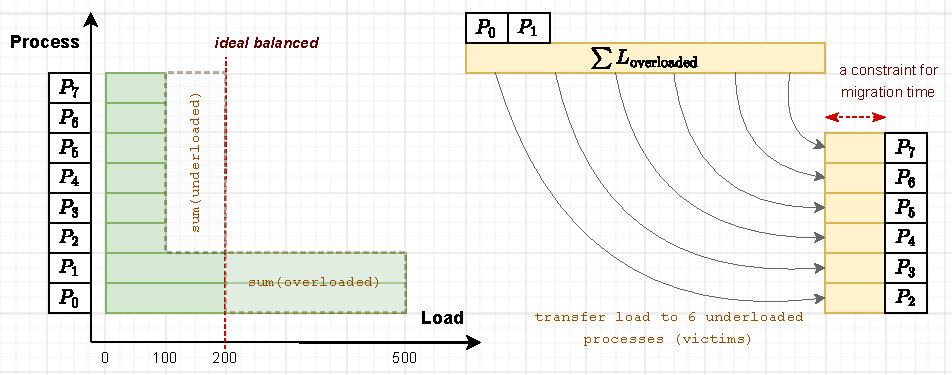
\includegraphics[scale=0.65]{./pictures/perf_analysis_model/perf_analysis_avg_bound_principle_case_1.5_two_sld_procs.pdf}
	\caption{An illustration of deterministic estimation on average.}
	\label{fig:explain_avg_bound_for_situation_1}
\end{figure}

This scenario is illustrated in Figure \ref{fig:explain_avg_bound_for_situation_1}. The chart on the left side shows $8$ processes from $P_{0}$ to $P_{7}$ along with their total load values. The $L_{avg}$ value is determined by the dashed line, \textit{ideal balanced}. The chart on the right side highlights the total overloaded value of process $P_{0}$ and process $P_{1}$, which is fairly shared to $6$ underloaded processes, $M=6$. Hence, we can estimate how much time and how many tasks ($K$) are limited for migration. The scenario here represents the number of overloaded processes smaller than the number of underloaded processes, $P_{\text{overloaded}} < P_{\text{underloaded}}$.\\

% --------------------------------------------------------
\newpage
% --------------------------------------------------------

Expanding this scenario, we emphasize two more scenarios that are summarized as follows.

\begin{itemize}
	\item Scenario 1: is explained above and shown in Figure \ref{fig:explain_avg_bound_for_situation_1}. The slowdown factor is $5\times$, the number of slowed down processes is $2$, and $R_{imb} = 1.5$. This scenario shows the number of overloaded processes smaller than the number of underloaded processes, $P_{\text{overloaded}} < P_{\text{underloaded}}$.
	\item Scenario 2: the slowdown factor is also $5\times$, the number of slowed down processes is $4$, $R_{imb} = 0.7$, and $P_{\text{overloaded}} = P_{\text{underloaded}}$.
	\item Scenario 3: the slowdown factor is set $\approx 8\times$, the number of slowed down processes is $6$, $R_{imb} = 0.3$, and $P_{\text{overloaded}} > P_{\text{underloaded}}$.
\end{itemize}

The corresponding latency and bandwidth information is collected from three different HPC clusters. We use the average $\lambda$ and $\overline{B}$ measured from CoolMUC2\footnote{https://doku.lrz.de/display/PUBLIC/CoolMUC-2 \label{footnote:lrz_coolmuc}}, SuperMUC-NG\footnote{https://doku.lrz.de/display/PUBLIC/SuperMUC-NG \label{footnote:lrz_sng}}, and BEAST\footnote{https://www.lrz.de/presse/ereignisse/2020-11-06\_BEAST/ \label{footnote:lrz_beast}} at Leibniz Supercomputing Centre (LRZ). These systems are also used to perform experiments in the following sections. CoolMUC2 has 28-way Intel Haswell-based nodes and an FDR14 Infiniband interconnect. SuperMUC-NG features Intel Skylake compute nodes with 48 cores per dual-socket, using Intel OmniPath interconnection. In BEAST system, the compute nodes are connected via a higher interconnect bandwidth, HDR 200Gb/s InfiniBand.\\

\begin{figure}[t]
  \centering
  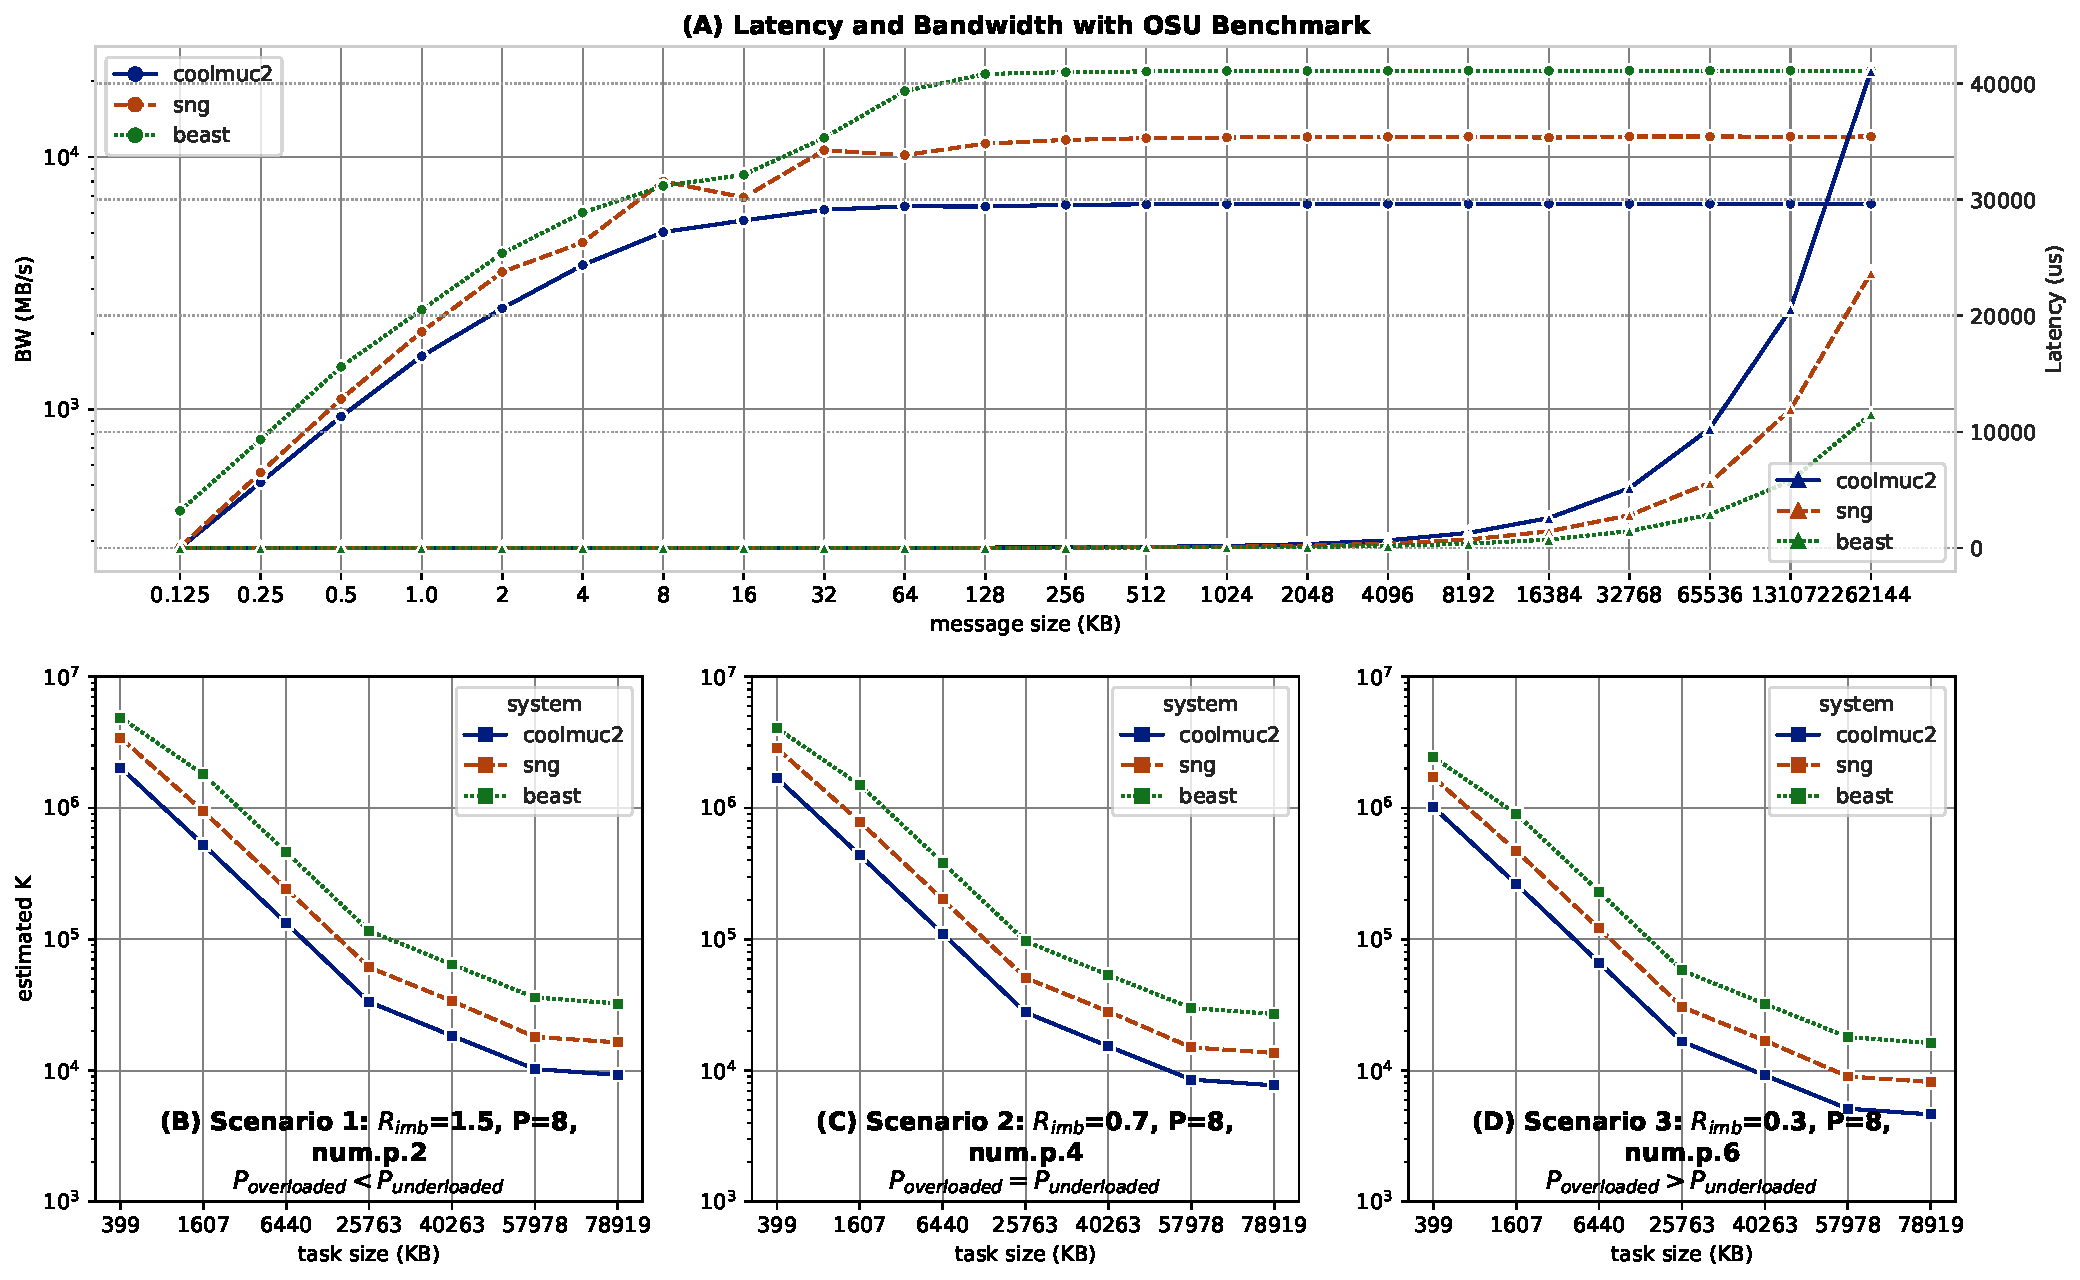
\includegraphics[scale=0.4375]{./pictures/perf_analysis_model/perf_k_offload_tasks_vs_delay_avg_bound.pdf}
	\caption{Estimation of $K$ offloaded tasks on average under the constraints of delay time, imbalance level, task data size, and the number of slowdown processes in task migration.}
	\label{fig:k_estimation_avg_bound}
\end{figure}

The average latency $\lambda$ and bandwidth $\overline{B}$ of CoolMUC2 (\texttt{coolmuc2}), SuperMUC-NG (\texttt{sng}), and BEAST system (\texttt{beast}) are shown in Figure \ref{fig:k_estimation_avg_bound} (A), measured by OSU Benchmark \cite{panda2021mvapich}. The benchmark is run on each cluster with two nodes, and the basic communication interface is MPI point-to-point. The x-axis shows message sizes from 128 bytes to 256 MB that can account for the data size of tasks during migration. The left y-axis shows bandwidth in $MB/s$, while the right y-axis shows latency in $\mu$s. As a result, BEAST has the best communication performance, while CoolMUC2 is the worst due to different interconnection technologies. \\

In Figure \ref{fig:k_estimation_avg_bound} (B), (C), (D), we show the results of $K$ estimation associated with the mentioned scenarios $1$, $2$, $3$. Following the x-axis, we show the task sizes from $400$ KB to $78919$ KB (almost $80$ MB), which are enough to highlight the trend of $K$ estimation and to represent the data sizes of each task in common task-based parallel applications. The y-axis shows the $K$ values, representing the maximum number of tasks that we can offload under the constraints of $\sum L_{\text{overloaded}}$, $\lambda$, and $M$. In Figure \ref{fig:k_estimation_avg_bound} (B), $R_{imb}$ is $1.5$, and two processes are slowed down. The total overloaded value is from process $P_{0}$ and process $P_{1}$, where we share this amount of load over $6$ victim processes. We highlight that the migration time of tasks should not exceed the shared value shown as the constraint segment over migration time in Figure \ref{fig:explain_avg_bound_for_situation_1}.\\

Similarly, Figure \ref{fig:k_estimation_avg_bound} (C) and (D) show that $K$ is decreased when the data size of tasks increases. The value of $K$ still reaches thousands tasks if we offload the tasks continuously, in particular with the size $\approx$ $80$ MB. This shows that communication overhead for task migration in distributed memory might not be the most influential factor. There might be some impacts from the other factors in balancing operations before a task can be migrated. Besides that, $K$ estimated in this bound relies on the average of accumulative overloaded and underloaded values. In the following paragraph, $K$ estimation is conducted in the bound of maximum overloaded and minimum underloaded values, which might stretch the constraint segment of migration time and $K$ may be more than the average bound. \\

\begin{figure}[t]
  \centering
  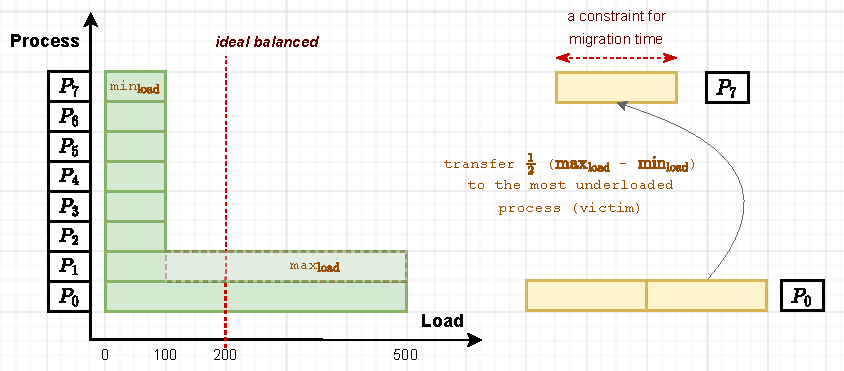
\includegraphics[scale=0.65]{./pictures/perf_analysis_model/perf_analysis_minmax_bound_principle_case_1.5_two_sld_procs.pdf}
	\caption{An illustration of deterministic estimation on min-max load values.}
	\label{fig:explain_minmax_bound_for_situation_1}
\end{figure}

\noindent \textbf{Min-Max Bound:} simply revolves around the maximum (max) and minimum (min) load values of corresponding processes. Min-max implies the longest way to offload tasks between the most overloaded and the most underloaded processes. Their difference can represent the effect of delay time in task migration.\\

Figure \ref{fig:explain_minmax_bound_for_situation_1} illustrates estimating $K$ based on the most overloaded and underloaded process. The longest way is between process $P_{0}$ and process $P_{7}$, which dominates the most time progress for offloading tasks. Then, we cut a half of the load difference to share each other. The min-max bound of estimating $K$ is summarized as follows.

\begin{itemize}
	\item The difference between the min and max load values is denoted by $\Delta_{max-min} = L_{max} - L_{min}$.
	\item Based on $\Delta_{max-min}$, we estimate $K$ as the number of offloaded tasks. Similarly, the assumption about data size in migrating tasks is kept the same as average bound.
	\item  The bound of $K$ is calculated by
\end{itemize}

\begin{equation} \label{eq:minmax_bound}
	\begin{cases}
		K \times (\lambda + \frac{\overline{s}}{\overline{B}}) &\leq \frac{\Delta_{max-min}}{2} \\
		\Leftrightarrow K  &\leq \frac{\Delta_{max-min}}{2 \times (\lambda + \frac{\overline{s}}{\overline{B}})} \\
		\Leftrightarrow K  &\leq \frac{\Delta_{max-min} \times \overline{B}}{2 \times (\lambda \times \overline{B} + \overline{s})}
	\end{cases}
\end{equation}

\begin{figure}[t]
  \centering
  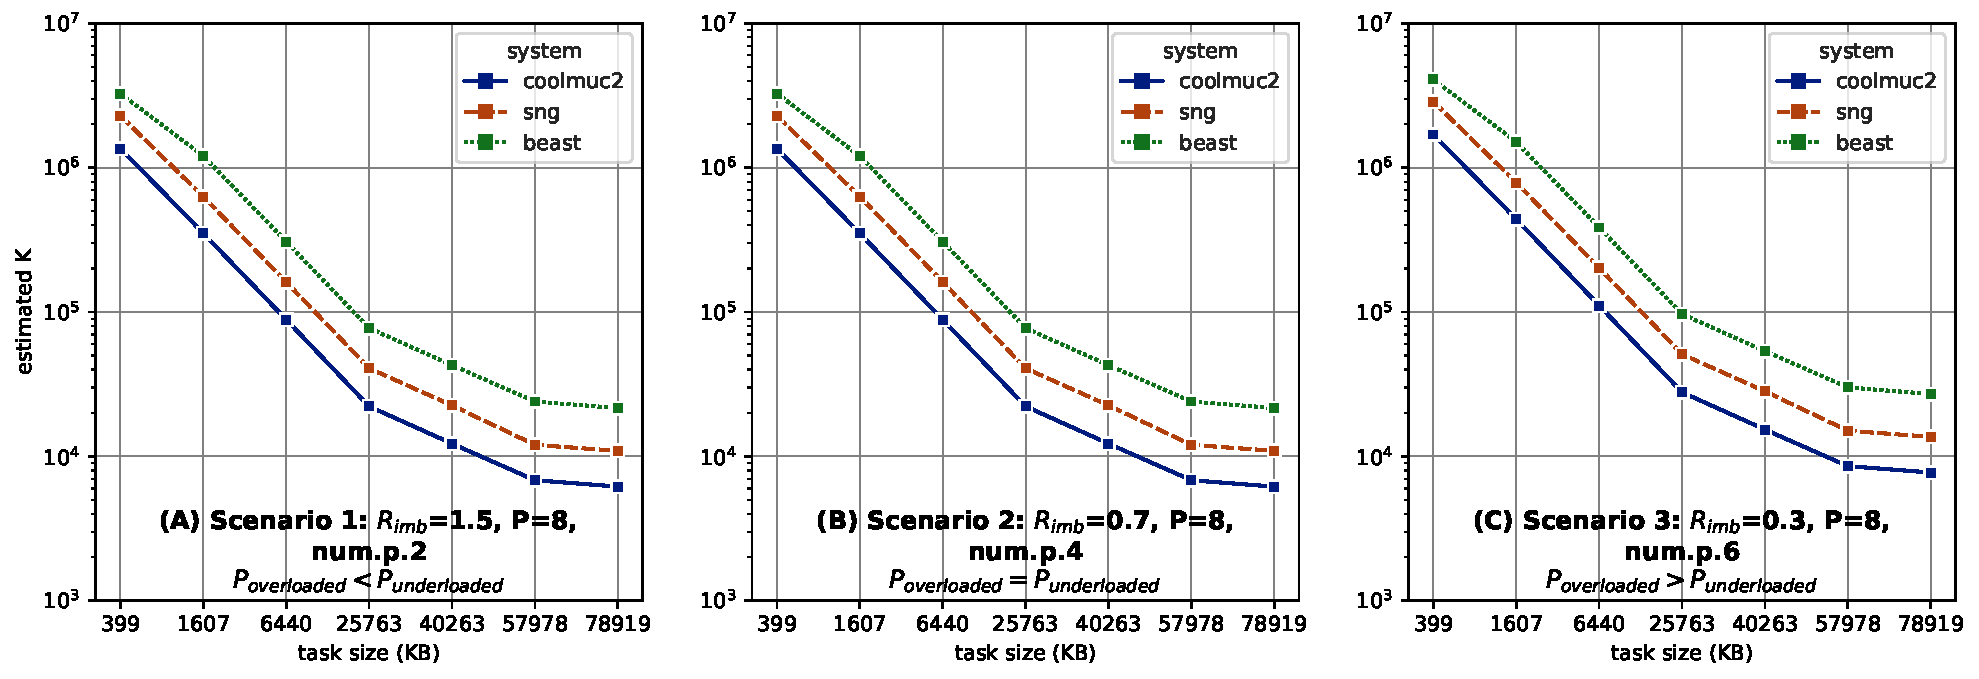
\includegraphics[scale=0.4375]{./pictures/perf_analysis_model/perf_k_offload_tasks_minmax_bound.pdf}
	\caption{The estimation of $K$ offloaded tasks under the constraints of delay, imbalance level, and task size with the bound of min-max load difference.}
	\label{fig:k_estimation_minmax_bound}
\end{figure}

The results of $K$ estimation are revealed in Figure \ref{fig:k_estimation_minmax_bound}. With the given latency and delay time on three corresponding clusters, the bound of $K$ is higher than the average bound. Likewise, $K$ is still high if we continuously perform offloading tasks during execution.\\

In practice, most analyses and hypotheses suggest that the impact of communication overhead on task migration contributes to slow work stealing as well as reactive load balancing. However, we show that task migration overhead is not only the most influential factor if we perform offloading tasks continuously. These estimations motivate a more in-depth analysis between task migration overhead and balancing operation overhead. The overhead of balancing operations includes the time of monitoring load, exchanging information, and calculating imbalance ratio before we decide to offload a task. The following subsection will show how they impact task offloading decisions.

% On the side of dedicated threads, $Tcomm_{i}$ is bounded by the bottleneck process with the maximum load. With $T_{\text{offload}}$ we can estimate the number of offloaded tasks ($K$) as an upper bound for $\sum_{k=0}^{K} w_{k}^{\text{remote}}$.

% The idea is to see, in general, how many tasks can be offloaded and how much balance we can improve with the given information. Following this, we briefly recall the context in this thesis alongside. The problem gives $T$ tasks in total distributed on $P$ processes. After a distribution, each process is assigned a set of tasks, $T_{i}$ for process $i$. Corresponding to $T_{i}$, the total load of each process is $L_{i}$. To facilitate modeling, we define each task belonging to a set $T_{i}$ with a weight of execution time $w_{j}, \forall j \in T_{i}$. In the case of non-interference during execution, the total load per process is $L_{i} = \sum_{j \in T_{i}} w_{j}$.\\

%As we can see, the context of unexpected imbalance looks simple. However, many factors can make it difficult to work at runtime, e.g., the level of ($R_{imb}$), the number of underloaded or overloaded processes, task data in migration, delay time. Step by step, the deterministic model estimates the performance as follows,
%\begin{enumerate}[label=\arabic*)]
%	\item Given $P$ processes, $T$ tasks in total.
%	\item Following a given distribution, each process holds a set $T_{i}$ tasks corresponding to a total load value $L_{i}$, where $\forall i \in P$.
%	\item For performance slowdown at runtime, $L_{max}$, $L_{min}$, $L_{avg}$ are defined as the maximum, minimum, and average load respectively. The imbalance ratio is calculated by $R_{imb} = \frac{L_{max}}{L_{avg}} - 1$, where $L_{max}$ is considered to define the makespan or completion time.
%	\item Without load balancing, the performance model on each process is $L_{i} = \sum_{j \in T_{i}} w_{j}$. The $L_{i}$ value indicates the load of local tasks belonging to the original process.
%	\item With load balancing, the communication thread ($Tcomm_{i}$) runs along with the other execution threads to monitor load and offload tasks. It partially overlaps communication \& computation. Therefore, we also count it inside the model. The average load value ($L_{avg}$) is concerned as an optimal value of balance. Reactively, tasks from the \textit{overloaded} rank (who has load $> L_{avg}$) are offloaded to the corresponding \textit{underloaded} rank (who has load $< L_{avg}$). Following that, we define the model below.

%			Inside $Tcomm_{i}$, we spend time or so-called overhead for monitoring load/execution speed ($T_{\text{monitor}}$), task offloading ($T_{\text{offload}}$), and monitored information exchange ($T_{\text{info\_exchange}}$). The inline figure shows why we have these terms in the model. The idea comes from the behavior of reactive task offloading or even work stealing. Before a task is migrated, we have to perform several operations, e.g., check the status, share information, and calculate the imbalance condition. They also take time to manage and might lead to late decision-making. Each process has a dedicated $Tcomm_{i}$, which runs along with the main execution. Therefore, $L_{i}$ will be affected when task offloading happens or imbalance conditions meet. Besides, these reactive operations occur repeatedly and dynamically that might show: $T_{\text{monitor}}$, $T_{\text{info\_exchange}}$, $T_{\text{offload}}$ slots are interleaved. The task offloading is unlikely to satisfy the condition to occur continuously.
%\end{enumerate}

%However, the imbalance problem might happen at runtime because of performance slowdown on some processors. For applying reactive load balancing, one dedicated thread per process will run asynchronously with the other execution threads. To model this behavior, we assume discrete execution time regulated by steps such as a time unit.
%
%The communication in HPC systems is challenging to predict how the variability changes. A part of this is due to the physical and virtual distance between nodes in large-scale distributed computing systems. Communication and task transfer activity among them cannot be assumed instantaneous. Thus, the information that a particular node has about other nodes at any time is dated and may not accurately represent the current state of the other nodes.\\
%
%The previous section shows a related performance model for work stealing and latency. The authors highlight how the latency can impact an upper bound of optimizing makespan. Nevertheless, there are still further problems with delay time in practice. Besides, we also need further analysis in modern architectures and new parallel programming paradigms. In detail, we address some opinions to motivate our proposed performance model as follows.
%\begin{itemize}
%	\item The existing models focus on latency which is considered as a constant time between sending and receiving the head of a message. This might imply that the migration time of tasks will be the same, not completely reflected in practice. Because we consider task migration time to be affected by latency, bandwidth, and message size at a time. If there are no conflicts, the transmission time (delay $d$) can be calculated by $d = \lambda + \frac{s}{B}$, where $d$ is delay, $\lambda$ is latency, $s$ and $B$ are message size, network bandwidth.
%	\item In terms of modern architectures and current programming models such as task-based paradigms, a process can have multiple execution threads, and one can be dedicated to communication. This paradigm can overlap communication and computation overhead. The dedicated thread can reduce time delay and perform asynchronously while other threads execute tasks. However, its behavior might be incorrect just due to the time delay in deciding the victim and tasks for offloading.
%\end{itemize}
%
%The above opinions generally motivate us to a performance model for work stealing or reactive load balancing approaches with delay time. ``Reactive'' means that we do not need to wait for the idle processes, and tasks will be considered for migration in advance. Therefore, we call reactively offload tasks from a slow process to a fast one asynchronously if an imbalance condition meets. The reactive idea can work in a distributed memory system. This section will mainly focus on reactive fashion and introduce a new model to analyze it. The model's target is to estimate an upper bound of task offloading under the input constraints of imbalance level, number of task distribution, and delay in task offloading. Figure \ref{fig:perfmodel_reactlb_behavior} shows again the illustration of reactive load balancing with task offloading behaviors.\\
%
%\begin{itemize}
%	\item Each process has a dedicated thread that monitors execution speed and offloads tasks around when the imbalance condition is met.
%	\begin{itemize}
%		\item Execution speed monitoring: this information depends on how we define it. Traditionally, we count the number of remaining tasks per queue to get the status of each process (or so-called MPI rank). The values reflect $T_{i}(t)$ at time $t$.
%		\item Imbalance condition: we can also rely on $T_{i}(t)$ at a time to calculate $R_{imb}$ if there is no prior knowledge about load.
%	\end{itemize}
%	\item Number of offloaded tasks at a time: without prior knowledge, this value can be set based on a specific strategy. For a safe threshold, it should be one task at once. Therefore, $O_{ij}(t) = 1$ indicates that Process $i$ offloads $1$ task to $j$ at time $t$.
%	\item $Tcomm$ should terminate after the bottleneck process (which holds $W_{par}$ or the makespan) finishes.
%\end{itemize}
%
%To ease modeling, we approach two ways of model formulation. One is a deterministic model based on the assumption about the given distribution of tasks over processes without time progress. The other is a discrete-time model, including a decreased function of the queue length over time on each process.

% ----------------------------------------------------------
% Remarked questions or emaphasized hypothesis/opinions
% ----------------------------------------------------------
%\begin{shaded}
%	\noindent How performance slowdown impact imbalance ratio?
%\end{shaded}

% ----------------------------------------------------------
% Remarked questions or emaphasized hypothesis/opinions
% ----------------------------------------------------------
%\begin{shaded}
%	\noindent How does the average bound work with real system information?
%\end{shaded}

% ----------------------------------------------------
% Discrete Time Model in detail
% ----------------------------------------------------
\subsection{Discrete Time Model} \label{subsec:discrete_time_model}

The idea of discrete-time models is to break execution time progress into time steps. In our work, we aim to model the behaviors of reactive load balancing based on queue length over time steps. There are time variables and non-time variables. The values of non-time variables will jump from one value to another depending on how time moves along. The queue length of each process is denoted by $Q_{i}(t)$, where $i$ means process $P_{i}$. The queue length is decreased over a certain number of time steps indicated by $\Delta t$. With task offloading, the queue of a process might receive tasks or also send tasks to others. In principle, the queue length status is changed during execution, mainly following three operations shown in Figure \ref{fig:detailed_Tcomm_operations_and_L} on Page \pageref{fig:detailed_Tcomm_operations_and_L}. To be intuitive, we illustrate these operations through process $P_{i}$ and process $P_{j}$ in Figure \ref{fig:anatomy_react_events}.\\

\begin{figure}[t]
  \centering
  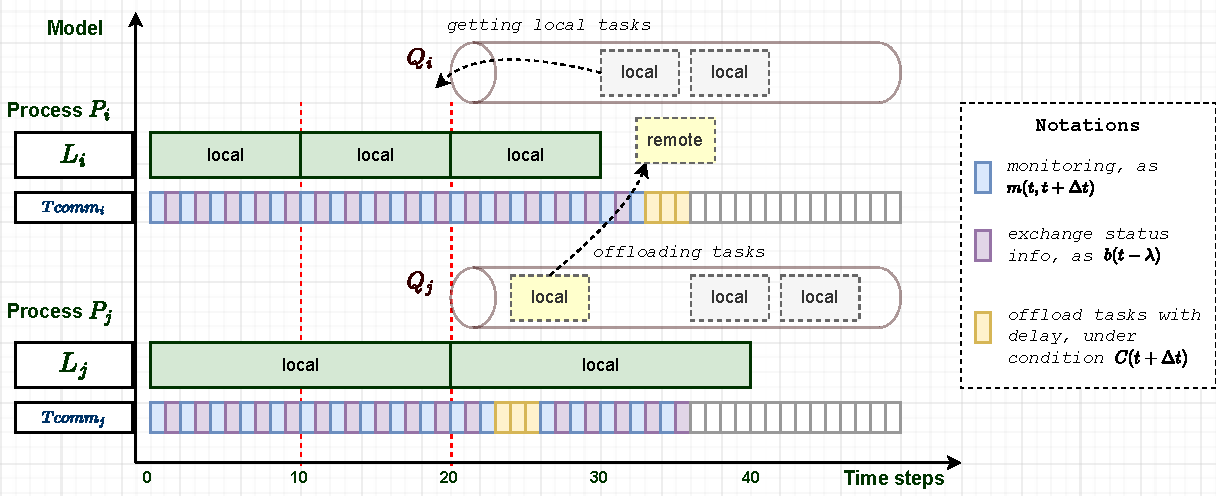
\includegraphics[scale=0.65]{./pictures/perf_analysis_model/perf_discrete_time_model.pdf}
	\caption{An anatomy of reactive load balancing events over discrete time steps.}
	\label{fig:anatomy_react_events}
\end{figure}

The y-axis shows each process with the label of total load values ($L_{i}$, $L_{j}$) and dedicated communication threads ($Tcomm_{i}$, $Tcomm_{j}$). The x-axis points to the execution progress over time steps, where we can see reactive balancing operations on $Tcomm$, for example, task execution, actions on each queue such as enqueuing tasks, offloading tasks. A task offloaded from its original queue (\texttt{local}) to another is called a remote task (\texttt{remote}). Our model is presented as follows (in Equation \ref{eq:react_model}).

\begin{equation} \label{eq:react_model}
	\begin{cases}
		& Q_{i}(t + \Delta t) = Q_{i}(t) - \mu_{i}(t, t+\Delta t) - \sum_{i \neq j} O_{ij}(t) + \sum_{j \neq i} O_{ji}(t -d_{ji}) \\ 
		& C_{i}(t + \Delta t) = \frac{Q_{max} - Q_{min}}{Q_{max}}, C_{i}(t + + \Delta t) > \text{const}(R_{imb}) \\
		& M_{i}(t + \Delta t) = m_{i}(t, t+\Delta t) + b_{i}(t - \lambda) \\
		& Tc_{i}(t + \Delta t) = Tc_{i}(t) + \Delta(t)
	\end{cases}
\end{equation}

The parameters of the model are driven by:

\begin{itemize}
	\item $Q_{i}(t + \Delta t)$: indicates the queue length status varied over a number of $\Delta t$ time steps. Alternatively, we can say that $t + \Delta t$ addresses the changes of queue $Q_{i}$ of process $P_{i}$ in the interval $(t, \Delta t]$. In response to $Q_{i}$ at $t + \Delta t$, the status at the previous step ($t$) is affected by $\mu_{i}(t, t+\Delta t)$ (task execution rate), $\sum_{i \neq j} O_{ij}(t)$ (the number of offloaded tasks from process $P_{i}$ to another, i.e., process $P_{j}$), and $\sum_{j \neq i} O_{ji}(t - d_{ji})$ (the number of remote tasks that process $P_{i}$ received from another, i.e., process $P_{j}$).
	
	\item $\mu_{i}(t, t+\Delta t)$: represents how many tasks are executed in a period of $\Delta t$. For instance, there could be 2, 3, ... tasks finished.
	
	\item $\sum_{i \neq j} O_{ij}(t)$: indicates the number of offloaded tasks from process $P_{i}$ to $P_{j}$, leading its sign negative. $\sum_{j \neq i} O_{ji}(t - d_{ji})$ indicates the number of remote tasks received from process $P_{j}$. Additionally, sending tasks from process $P_{i}$ to process $P_{j}$ is performed asynchronously by the dedicated thread, and during migration, the other threads still execute local tasks. Therefore, we do not count delay time for sending tasks. In contrast, receiving tasks at the side of process $P_{i}$ from process $P_{j}$ affects task execution on process $P_{i}$ if the delay time is taken into account. This is why we need the term of $d_{ji}$ in $\sum_{j \neq i} O_{ji}(t - d_{ji})$, and its sign is positive.
	
	\item $C_{i}(t + \Delta t)$: models when the imbalance condition is checked and met. Notably, the values of $\sum_{i \neq j} O_{ij}(t)$ and $\sum_{j \neq i} O_{ji}(t - d_{ji})$ depend on when an imbalance is detected and when reactive load balancing takes decision. Corresponding to the strategy of reactive task offloading, an imbalance condition is met when the queue length ratio is satisfied with a given constant of $R_{imb}$. The returned value of $C_{i}(t + \Delta t)$ at a time is $0$ or $1$, which means ``balanced'' or ``unbalanced''.
	
	\item $M_{i}(t + \Delta t)$: models the operations of monitoring load and exchanging load. Each process needs load information to calculate $C_{i}(t + \Delta t)$. The current length of queues represents the load information here. Therefore, $M_{i}(t + \Delta t)$ is used to model the action of monitoring and exchanging load, denoted by $m_{i}(t, t+\Delta t)$ and $b_{i}(t - \lambda)$ respectively. Unlike the data size of tasks, each action of exchanging information is modeled with latency because the size of load information is supposed to be small as sending and receiving the header of a message.
	
	\item $Tc_{i}(t + \Delta t)$: is considered as the time clock and represents the dedicated thread, $Tcomm$. In this model, we use $Tc_{i}$ to indicate clocking (counting time steps).
	
\end{itemize}

\noindent To illustrate how the model in Equation \ref{eq:react_model} works, we reuse the example illustrated in Figure \ref{fig:anatomy_react_events}. Following the operations of $Tcomm$, their notations on the right side show the corresponding parameters of the model. Different colors distinguish different operations. For example, the blue boxes illustrate monitoring load modeled by $m_{i}(t, t+\Delta t)$, the violet boxes illustrate load information exchange ($b_{i}(t - \lambda)$ ), and the orange ones illustrate offloading tasks under the condition of $C_{i}(t + \Delta t)$.\\

Starting at time $t = 0$, we assume $5$ tasks per process. The execution speed on process $P_{j}$ is slower than process $P_{i}$, $\mu_{i} = 2 \mu_{j}$, leading to an imbalance.
\begin{itemize}
	\item At $t=10$, we have $Q_{i} = 4 - 1 - 0 + 0$, $Q_{j} = 4 - 0 - 0 + 0$, $M_{i} = M_{j} = Tc_{i} = Tc_{j} = 10$, where $M_{i}$ and $M_{j}$ just have the overhead of monitoring load ($m_{i}$, $m_{j}$). 
	\item At $t=20$, we have $Q_{i} = 3 - 1 - 0 + 0$, $Q_{j} = 4 - 1 - 0 + 0$. With the current status at $t = 20$, Process $j$ meets the imbalance condition. Then, it exchanges this information at $t = 21$, and one task is offloaded reactively at $t = 23$.
\end{itemize}

In practice, delay time depends on the data size of tasks; therefore, offloading different tasks might have different delays. Besides, the values of latency ($\lambda$) and delay time ($d$) might fluctuate at runtime. For example, the offloaded task from process $P_{j}$ to process $P_{i}$ is started asynchronously at $t=23$; then it arrives on the side of process $P_{i}$ at $t=33$ if we assume delay $d_{ji}$ takes $10$ time steps. Simultanously, $d_{ji}$ might be varied in practice such as $12$, $13$, etc. Our discrete-time model is intended to simulate reactive load balancing in particular and dynamic load balancing behaviors in general. The following section will show how we design a simulator and evaluate it.

%Technically, the runtimes support distributed memory. The program has multiple processes; each spawns multiple threads for executing tasks\footnote{Basically, we consider the model of $P$ involved processes, not the number of compute nodes. Because a compute note might have multiple processes, depending on NUMA domain. Usually, there are two or four processes (so-called MPI ranks) per node.}. One thread is dedicated to performing communication ($Tcomm$). The model of each process will be formulated by the decrease of its queue length, $Q_{i}(t)$, over time steps ($\Delta t$). $Tcomm$ runs asynchronous with the main execution threads; therefore, we consider it as a time clock in this model. However, the $Tcomm$ actions are involved, and they affect the queue length. The model is detailed as follows: each variable points to the current time step and implies the change with the previous step by $\Delta t$.